% !TeX encoding = UTF-8
% !TeX program = xelatex
% !TeX spellcheck = en_US

\documentclass[degree=bachelor]{ustcthesis}
% degree      = doctor | master | bachelor
% degree-type = academic | professional
% language    = chinese | english
% fontset     = windows | mac | ubuntu | fandol

% 加载宏包、全部的配置
% !TeX root = ./main.tex

\ustcsetup{
  title              = {云闪存系统中的多租户性能隔离研究},
  title*             = {Multi-tenant Performence Isolation in Cloud-based Flash Storage Systems},
  author             = {樊金昊},
  author*            = {Jinhao Fan},
  speciality         = {计算机科学与技术},
  speciality*        = {Computer Science and Technology},
  supervisor         = {程鹏~首席研究员, 李诚~特任研究员},
  supervisor*        = {Dr. Peng Cheng, Prof. Cheng Li},
  % date               = {2017-05-01},  % 默认为今日
  % professional-type  = {专业学位类型},
  % professional-type* = {Professional degree type},
  % secret-level       = {秘密},     % 绝密|机密|秘密,注释本行则不保密
  % secret-level*      = {Secret},  % Top secret|Highly secret|Secret
  % secret-year        = {10},      % 保密年限
  %
  % 数学字体
  % math-style         = GB,  % 可选:GB, TeX, ISO
  math-font          = xits,  % 可选:stix, xits, libertinus
}


% 加载宏包

% 定理类环境宏包
\usepackage{amsthm}

% 插图
\usepackage{graphicx}

% 三线表
\usepackage{booktabs}

% 跨页表格
\usepackage{longtable}

% 算法
\usepackage[ruled,linesnumbered]{algorithm2e}

% SI 量和单位
\usepackage{siunitx}

% 参考文献使用 BibTeX + natbib 宏包
% 顺序编码制
\usepackage[sort]{natbib}
\bibliographystyle{ustcthesis-numerical}

% 著者-出版年制
% \usepackage{natbib}
% \bibliographystyle{ustcthesis-authoryear}

% 本科生参考文献的著录格式
% \usepackage[sort]{natbib}
% \bibliographystyle{ustcthesis-bachelor}

% 参考文献使用 BibLaTeX 宏包
% \usepackage[style=ustcthesis-numeric]{biblatex}
% \usepackage[bibstyle=ustcthesis-numeric,citestyle=ustcthesis-inline]{biblatex}
% \usepackage[style=ustcthesis-authoryear]{biblatex}
% \usepackage[style=ustcthesis-bachelor]{biblatex}
% 声明 BibLaTeX 的数据库
% \addbibresource{bib/ustc.bib}

% 配置图片的默认目录
\graphicspath{{figures/}}

% 数学命令
\makeatletter
\newcommand\dif{%  % 微分符号
  \mathop{}\!%
  \ifustc@math@style@TeX
    d%
  \else
    \mathrm{d}%
  \fi
}
\makeatother
\newcommand\eu{{\symup{e}}}
\newcommand\iu{{\symup{i}}}

% 用于写文档的命令
\DeclareRobustCommand\cs[1]{\texttt{\char`\\#1}}
\DeclareRobustCommand\pkg{\textsf}
\DeclareRobustCommand\file{\nolinkurl}

% hyperref 宏包在最后调用
\usepackage{hyperref}

\usepackage{caption}
\usepackage{subcaption}
\usepackage{pifont}% http://ctan.org/pkg/pifont
\newcommand{\cmark}{\checkmark}%
\newcommand{\xmark}{\ding{53}}%
\newcommand{\JF}[1]{[\textcolor{red}{JF: #1}]}  % Jinhao Fan

\begin{document}

% 研究生论文:
%   封面,原创性声明和授权使用声明
%   frontmatter: 摘要,目录,[图、表清单],[符号说明]
%   mainmatter: 正文章节,参考文献
%   appendix: 附录
%   backmatter: 致谢,已发表论文列表
%
% 本科生论文:
%   封面
%   frontmatter: 致谢,目录,摘要
%   mainmatter: 正文章节,参考文献
%   appendix: 附录

\maketitle
\copyrightpage

\frontmatter
% !TeX root = ../main.tex

\begin{acknowledgements}

我的毕业设计是在微软亚洲研究院实习期间完成的,期间有幸得到了杨子岳、舒然、程鹏、熊勇强、周礼栋、曹婷等研究员的指导。
微软亚洲研究院的学术气氛和研究员们对各自领域的深入理解都让我受益良多。
在工作之余,我还获得了很多和研究员以及其他实习生交流的机会,从这些“大牛”的成长经历中收获了对人生前途的思考,可谓不虚此行。

除此之外,在完成毕业设计的过程中,我还得到了校内导师李诚老师的热情帮助。
感谢在科大期间在课程和其他方面指导过我的老师们,他们身上严谨、务实的“孺子牛”精神为我打下了深深的科大烙印。

\end{acknowledgements}
\tableofcontents
% !TeX root = ../main.tex

\ustcsetup{
  keywords = {
    中国科学技术大学, 学位论文, \LaTeX{} 模板, 学士, 硕士, 博士
  },
  keywords* = {
    University of Science and Technology of China (USTC), Thesis,
    \LaTeX{} Template, Bachelor, Master, PhD
  },
}

\begin{abstract}
  摘要分中文和英文两种,中文在前,英文在后,博士论文中文摘要一般 800~1500 个汉字,硕士论文中文摘要一般 500~1000 个汉字。
  英文摘要的篇幅参照中文摘要。

  关键词另起一行并隔行排列于摘要下方,左顶格,中文关键词间空一字或用分号“,”隔开,英文关键词之间用逗号“,”或分号“;”隔开。

  中文摘要是论文内容的总结概括,应简要说明论文的研究目的、基本研究内容、研究方法或过程、结果和结论,突出论文的创新之处。
  摘要应具有独立性和自明性,即不用阅读全文,就能获得论文必要的信息。
  摘要中不宜使用公式、图表,不引用文献。

  中文关键词是为了文献标引工作从论文中选取出来用以表示全文主题内容信息的单词和术语,一般 3~8 个词,要求能够准确概括论文的核心内容。
\end{abstract}

\begin{abstract*}
  This is a sample document of USTC thesis \LaTeX{} template for bachelor,
  master and doctor. The template is created by zepinglee and seisman, which
  orignate from the template created by ywg. The template meets the
  equirements of USTC theiss writing standards.

  This document will show the usage of basic commands provided by \LaTeX{} and
  some features provided by the template. For more information, please refer to
  the template document ustcthesis.pdf.
\end{abstract*}

% \listoffigures
% \listoftables
% % !TeX root = ../main.tex

\begin{notation}

  \begin{notationlist}{2em}
    \item[$\displaystyle a$] The number of angels per unit area
    \item[$\displaystyle N$] The number of angels per needle point
    \item[$\displaystyle A$] The area of the needle point
    \item[$\displaystyle \sigma$] The total mass of angels per unit area
    \item[$\displaystyle m$] The mass of one angel
    \item[$\displaystyle \sum_{i=1}^n a_i$] The sum of $a_i$
  \end{notationlist}

\end{notation}



% 也可以使用 nomencl 宏包

% \printnomenclature

% \nomenclature{$\displaystyle a$}{The number of angels per unit are}
% \nomenclature{$\displaystyle N$}{The number of angels per needle point}
% \nomenclature{$\displaystyle A$}{The area of the needle point}
% \nomenclature{$\displaystyle \sigma$}{The total mass of angels per unit area}
% \nomenclature{$\displaystyle m$}{The mass of one angel}
% \nomenclature{$\displaystyle \sum_{i=1}^n a_i$}{The sum of $a_i$}


\mainmatter
% !TeX root = ../main.tex

\chapter{绪论}
\label{chap:intro}

基于闪存的固态硬盘(SSD)正在数据中心中得到越来越广泛的应用。
与机械硬盘(HDD)相比,SSD的吞吐和访问延迟都有数量级的提升~\cite{chen2009understanding}。
特别地,由于内部存储介质不同,SSD的随机访问性能尤为出色。
因此,主流的云计算厂商,如Azure、AWS等,都提供了基于SSD的高性能存储服务~\cite{awsebs,azuredisks}。
专门针对固态硬盘进行优化的键值存储引擎RocksDB也得到了广泛的部署~\cite{cao2020characterizing,rocksdb,siying2021rocksdb}。

云闪存系统的服务质量往往是由吞吐、延迟等性能决定的。
对于云服务商而言,对于服务质量的保证是他们对租户的服务等级协议(SLA,Service Level Agreement)的一部分。
例如,AWS的io2 SSD服务,提供了500IOPS/GiB,最高达64KIOPS的吞吐~\cite{awsio2}。
近期的新存储服务,例如Azure Ultra Disk~\cite{azureultradisk},提供次毫秒级的延迟保证。
由于在分布式在线服务中,尾延迟受到了关注~\cite{dean2013tail},因此学术界也开始关注为SSD服务提供尾延迟保证~\cite{klimovic2017reflex}。

% 与此同时,为了解决数据中心资源利用率低的问题~\cite{kanev2015profiling},研究人员提出了资源池化(Resource Disaggregation)的方法~\cite{shan2018legoos,klimovic2016flash}。
% 通过将原本紧耦合的CPU、内存、硬盘等资源分别组织成独立的资源池,云服务商可以调度多租户共用物理资源,使有限的资源得到尽可能大的复用,避免浪费。
% 因此,资源池化在学术界和工业界都受到了广泛的关注。
% 目前,资源池化已经广泛地存在于云存储服务中。
% Azure Blob Storage~\cite{azureblob}、AWS S3~\cite{awss3}等对象存储服务
% 和Azure Disk Storage~\cite{azuredisks}、AWS Elastic Block Store~\cite{awsebs}等块存储服务
% 都提供了独立于计算服务的、多租户共享的存储抽象。

然而,想要在SSD上提供良好的SLA并不容易。
这是因为SSD的内在机制给服务质量带来了新的挑战——多租户间的性能隔离。
当多个租户共享同一块物理硬盘时,他们的访问性能不应相互影响。
这一保证在SSD上不易实现。
由于基于闪存的SSD的内在特性,共享同一块物理SSD的多个租户之一进行的写操作可能会触发SSD的垃圾回收、缓冲区清除等内部维护行为,这些行为将会影响其它租户的访问性能。
特别地,这一读写干扰~\cite{klimovic2017reflex}问题会使其它租户的访问尾延迟增加数倍。
对于追求快速响应的Web服务而言,这意味着其服务质量将受到较大的影响~\cite{dean2013tail}。
因此,追求低延迟的应用仍倾向于使用本地独占的SSD存储~\cite{awsvm,azurevm}。

\begin{figure}[h]
  \centering
  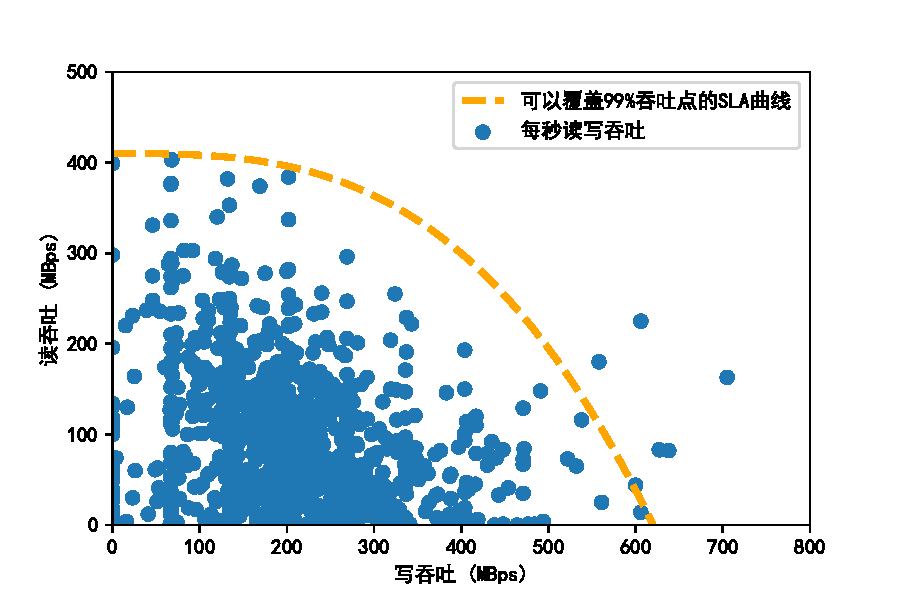
\includegraphics[width=0.8\textwidth]{thesis-intro-ycsb.pdf}
  \caption{
        YCSB负载A在RocksDB上运行时,每秒的读写吞吐没有固定的比例,且几乎不会同时达到最大的读和写吞吐,因此更适合用曲线描述其带宽需求。
      }
  \label{fig:intro}
\end{figure}

简单限制各个租户分享到的最大带宽的方式不能限制读写干扰,因此不能实现性能隔离。
并且,由于SSD的读写操作对磁盘的影响并不对称,需要同时考虑租户的读和写带宽。
事实上,租户在不同时间往往有不同的读写吞吐比例,他们的最大吞吐更适合用一条由不同读写带宽包围出的曲线表示。
\autoref{fig:intro}所示为~\citet{yadgar2021trace}采集的将YCSB负载A在RocksDB上运行得到的块请求记录,图中截取了其在10分钟每秒的读写吞吐。
由图可见,其读写吞吐在不同的比例之间变化,且几乎不会同时达到最大的读和写吞吐。

因此,本文使用\textit{SLA曲线}来描述服务质量。
具体来讲,SLA曲线表示的是在某个尾延迟要求下的最大读写带宽。
例如,\autoref{fig:intro}中的橙色虚线就可以作为以上YCSB负载的SLA曲线。
该曲线覆盖了99\%的读写吞吐,它基本代表了该负载对IO资源的需求。

针对以上问题,本研究搭建了一个具有多租户性能隔离功能的云闪存系统,该系统具有如下设计目标:
\textbf{1)高资源利用率}。
在云系统中,资源调度不再受限于“服务器”这一有限的单位。
本系统可以调度多租户共享同一物理硬盘上的存储空间和带宽,达到资源的高效利用;
\textbf{2)用户自定义SLA}。
在云闪存系统中,用户对存储资源的需求也不再受限于服务器上有限的资源。
本系统允许用户使用\textit{SLA曲线}定义其需要的读写带宽及达到该带宽时的尾延迟,系统会根据该定义为用户自动分配适合的存储硬盘。
\textbf{3)低尾延迟}。
本系统将各租户可保证的尾延迟作为存储性能隔离的评价指标。
通过减少或控制占用同一物理硬盘的各租户间的读写干扰,本系统可以降低各租户的尾延迟,从而实现有效的存储性能隔离。
\autoref{tab:cmp-ebs-insstore}中为本系统与目前主流云存储系统的对比。

\begin{table}[h]
  \centering
  \caption{本系统与常见云存储系统的对比}
  \label{tab:cmp-ebs-insstore}
  \begin{tabular}{cccc}
    \toprule
    \textbf{} & 高资源利用率 & 自定义SLA & 低尾延迟  \\
    \midrule
    传统池化存储系统 & \cmark & 部分 & \xmark  \\
    直连的闪存系统 & \xmark & \xmark & \cmark   \\
    \textbf{本系统} & \cmark & \cmark & \cmark  \\
    \bottomrule
  \end{tabular}
\end{table}

为了实现以上设计目标,本系统进行了如下设计。
首先,为了改善多租户读写干扰问题,本系统设计了无读写干扰的SSD阵列。
本系统提出\textit{分离的读写时间窗口},将对SSD的读写混合访问拆分为交替的纯读和批量写访问。
在纯读时间窗口中,本系统将所有写请求存于缓冲区中,从而获得无干扰的读性能;
纯写窗口中批量写入写请求,从而最大程度利用SSD的写带宽。
为了在纯写窗口中仍能服务读请求,本系统通过RAID~\cite{patterson1988case}或纠删码~\cite{huang2012erasure}等方式引入冗余。
通过协调不同硬盘中的时间窗口,使得所有数据总能被以无干扰的延迟被访问。

在此基础上,针对不同用户的不同SLA需求,本系统设计了基于SLA曲线的SSD资源分配算法。
本研究提出用SLA曲线定义用户的服务质量要求,并进一步定义了SLA曲线的加法、减法、包含等运算。
基于SLA曲线这一定义,本系统提出了一个多租户、多SSD数据分布的在线启发式算法。
该算法受向量装箱问题~\cite{panigrahy2011heuristics,hu2003operations}的启发,采用最佳适应算法,为系统中的租户提供了SLA保障,还得到了高效的资源利用率。
此外,本系统还实现了一个基于SLA曲线的IO请求调度器,它在运行时根据租户的实际吞吐,为每个租户提供SLA规定的吞吐和尾延迟保证。

本文的后续章节按如下方式组织:
第二章介绍本研究的动机——闪存资源池化系统中的多租户性能隔离问题,并介绍在保证SSD的服务质量方面的相关工作;
第三章介绍本研究所提出的系统设计,并详细介绍如何构建无读写干扰的冗余SSD阵列,以及基于背包问题的用户需求分配算法;
第四章介绍该系统的实现方式;
第五章通过大量实验证明了该系统的有效性;
第六章为本研究的总结。
% !TeX root = ../main.tex

\chapter{动机和背景}
\label{chap:background}

本章将介绍本研究的动机和相关背景。
\autoref{sec:bg-perf-isolation}将介绍云闪存系统中的多组合性能隔离问题重要性,
以及SSD的读写干扰问题及其产生的原因。
\autoref{sec:bg-related-work}将分别从硬盘本身和系统设计的层面介绍改进SSD存储系统服务质量的相关工作。

\section{云闪存系统中的多租户性能隔离问题}
\label{sec:bg-perf-isolation}

基于NAND介质闪存具有低延迟、高吞吐的特点,给存储系统带来了革命性的影响。
但是,对于云系统来说,只有当它能够稳定、可预测地提供以上特点时,基于闪存的SSD才能得到利用。
现代的虚拟化技术使得云系统中的多个租户可以共享同一个物理资源,却给每个租户独占该资源的假象~\cite{bugnion2017hardware}。
在这种抽象中,各个租户间的性能隔离对于满足租户的服务质量要求至关重要~\cite{somani2009isolation}。
若云系统的性能隔离不够充分,则每个租户随时可能受到其“吵闹的邻居”(Noisy Neighbor)的影响,其性能的稳定性将会受损。

在存储系统中,性能隔离主要指的是任一租户对物理资源访问的带宽和延迟基本不受其他租户的影响。
由于机械硬盘的延迟普遍较差,且读写性能差异不大,因此限制各个租户的带宽往往就可以实现多租户的性能隔离。
例如,Docker通过Linux的cgroup~\cite{cgroup}设置每个租户的带宽上限;
Ceph~\cite{weil2006ceph}也通过mClock~\cite{gulati2010mclock}设置虚拟时间,限制每个租户发送请求的频率,从而实现分布式的租户资源限制。

然而,交互性高的数据应用服务需要良好的存储尾延迟保证~\cite{dean2013tail,hao2016tail}。
这是因为现代云系统的分布式和并发特性,使得一个Web请求往往被同时分发到多个服务器上分别处理,该Web请求的响应时间将是这多个服务器的服务时间的最大值。
因此,若一个服务器响应时间的99\%分位数为2ms,则若一个请求被分发到100个服务器上处理,其响应时间的$0.99^{100}=36.6\%$分位数将为2ms。
也就是说,超过60\%的Web请求将经历尾延迟。
因此,某些用户除了对访问带宽有要求,还会要求对自己租用的SSD的读请求中99\%均有两毫秒以下的延迟。
尽管可以通过设置不同租户的优先级保证某些租户的请求被优先服务,但并不能给出严格的尾延迟保证。
在这种情况下,仅仅对每个用户的访问带宽进行限制是不够的。

\begin{figure}[h]
  \centering
  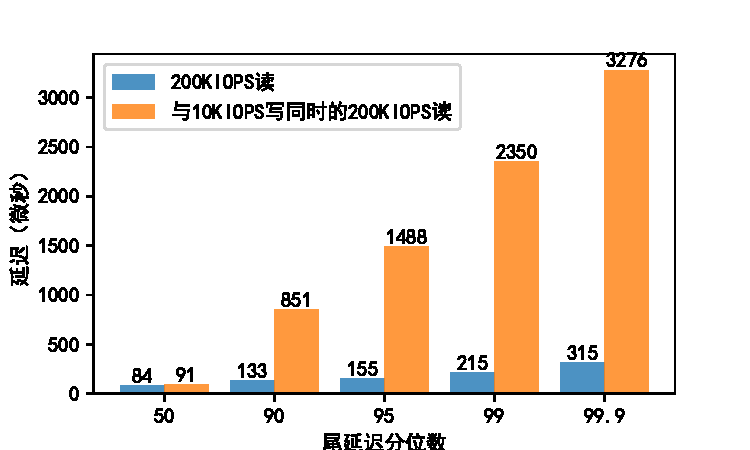
\includegraphics[width=0.8\textwidth]{thesis-wr-interfere.pdf}
  \caption{写操作对其他租户读延迟的影响。很小的写吞吐就使读租户的尾延迟增大了约10倍。}
  \label{fig:bg-wr-interfere}
\end{figure}

SSD内部的\textit{读写干扰}使多租户的性能隔离更加复杂。
对SSD的写操作可能会引起SSD内部的垃圾回收、缓冲区刷新等操作。
由于SSD内部的存储采用日志结构~\cite{ArpaciDusseau18-Book},因此对SSD中存储页的修改或删除并不会立即改变该页的内容,而只是将其标记为不再使用。
垃圾回收指的就是将不再使用的页回收起来准备之后使用,并把仍在使用的页合并在一起的过程。
此外,SSD为了最佳的写吞吐,会在内部维护写缓冲区,只有当缓冲区写满时才会将数据写入存储介质中。
缓冲区刷新指的就是上述写入存储介质的过程。
由于上述两种行为涉及对SSD内部的操作,因此同时进行的其它读写操作往往会被阻塞。

如\autoref{fig:bg-wr-interfere}所示,当一个租户在进行读操作时,另一个租户对不同位置的写操作是该租户的尾延迟增大了约十倍。
这就是由于上文提到的写操作触发的SSD内部的垃圾回收、缓冲区刷新等行为引起的。
当某个租户进行写操作时,SSD内部可能会进行针对某一区域的垃圾回收或缓冲区刷新,这些活动将会对该硬盘上其他租户的访问性能造成影响。
尽管这些活动并不常见,但这些异常的延迟却构成了租户的尾延迟。

\section{相关工作}
\label{sec:bg-related-work}

本节介绍在云闪存系统中提供服务质量保证的相关工作。
\autoref{sec:bg-related-work-ssd}将介绍如何在SSD层面提供服务质量的保证,
\autoref{sec:bg-related-work-system}将介绍在系统层面提供服务质量保证的方法。

\subsection{保证服务质量的SSD}
\label{sec:bg-related-work-ssd}

在SSD层面上提供服务质量的方式主要可分为两种。
第一种是对SSD的性能进行建模,从而预测垃圾回收、写缓冲区刷新等操作会在何时发生。
SSDCheck~\cite{kim2018ssdcheck}和FusionRAID~\cite{jiang2021fusionraid}通过一系列测试IO请求序列来获取SSD的垃圾回收间隔、写缓冲区大小等信息,
但是他们的测试脚本都基于对SSD行为的假设,在我们的实验中,并非所有SSD都遵循这一假设;
除此之外,ReFlex~\cite{klimovic2017reflex}利用曲线拟合,为SSD上的读写请求设定权重,后续每个租户的加权IOPS不能超过为其设定的限制;
近期,LinnOS~\cite{hao2020linnos}通过一个轻量的神经网络来预测每个请求的延迟是否会较大。

另一种方法是修改SSD控制器,使其具有控制服务质量的特性。
例如,NVMe 1.4标准~\cite{nvme2020}提出了I/O Determinism和NVM Set。
其中,I/O Determinism提供了具有确定性延迟和不确定性延迟的时间窗口,它规定了用户与SSD之间的一种协议。
SSD保证在确定性窗口中不进行后台的维护操作,用户则保证在确定性窗口中不进行写操作~\cite{petersen2018enabling}。
NVM Set是在SSD控制器层面就将资源拆分为多个集合,从而支持多个租户无干扰地共享同一SSD。
此外,还有其它通过修改SSD控制器~\cite{yan2017tiny,arash2018flin}和使用Open-Channel SSD来改进SSD的尾延迟的方法。

\subsection{保证服务质量的云服务系统}
\label{sec:bg-related-work-system}

如\autoref{sec:bg-perf-isolation}所述,传统的云存储服务大多以保证租户的吞吐为服务质量的优化目标~\cite{patterson2004latency, cgroup,gulati2010mclock}。
近年来,尾延迟越来越受到重视~\cite{dean2013tail},确保低尾延迟的一种常用方法是利用冗余。
% \JF{Performance Variablity?}

利用冗余的方法之一是负载均衡,即将每个请求尽可能分到负载最低的机器上,从而获得最好的响应时间。
有大量研究通过推断各个冗余服务器的负载来进行尽可能最优的请求分发。
例如,C3~\cite{suresh2015c3}通过估计队列深度和服务时间对冗余服务器进行排序来选择最优的冗余服务器。
\autoref{sec:bg-related-work-ssd}提到的对SSD进行性能建模的方式也可以用来进行冗余服务器的选择。

另一种利用冗余的方法是hedging,即将同一请求同时发给多个冗余服务器,并以其中最快的一个作为最终的结果。
在这种情况下,只有当所有冗余服务器均出现尾延迟时,该请求才会出现异常的高延迟,因此能将异常延迟出现的可能大大降低。
然而,这种方法会使各个服务器的负载增加~\cite{primorac2021hedge},因此并不能在所有情况下都确保比不使用冗余的尾延迟更好。
\citet{vulimiri2013low}通过排队论对利用冗余改善延迟进行了定量分析。

除此之外,还有一些系统试图在资源调度和集群管理时确保服务质量。
例如,PSLO~\cite{li2016pslo}利用控制论中的方法,实现了机械硬盘上的请求级尾延迟保证;
Quasar~\cite{delimitrou2014quasar}利用协同过滤预测租户所需的服务质量,并利用一个贪心算法选择最适合的资源配置方式。
% !TeX root = ../main.tex

\chapter{多租户性能隔离的闪存资源池化系统设计}

\section{隔离的读写时间窗口}

\section{闪存阵列}

\section{算法}
% !TeX root = ../main.tex

\chapter{系统实现}
\label{chap:impl}

如\autoref{chap:design}所述,本系统主要由三部分组成:控制器、客户端和存储单元。
他们的实现基于开源的Storage Performence Development Kit (SPDK)~\cite{yang2017spdk}工具和用于网络访问NVMe设备的NVMe-oF~\cite{nvmeof2016}等技术。

\section{控制器}
\label{sec:impl-controller}

本系统的控制器是用Python实现的,其职责是根据用户的请求,为其分配存储单元,并管理存储单元。
控制器通过RPC与客户端库和存储单元通信。
在本系统中,用户和存储单元的SLA曲线被采样后存放在数组中,SLA曲线的加、减等运算都在控制器中通过数组操作实现。
控制器存放着所有数据块的占有状态及从用户的地址空间到存储单元的地址空间的映射。
当需要启用新的存储单元时,控制器通过RPC告知存储服务器上的\JF{加内容}。

由于客户端库直接通过网络访问存储单元,所以为了数据的安全性,需要加入访问控制。
本系统在新租户加入系统时,由控制器生成token同时发送给租户和分配给它的存储单元。
只有当存储单元收到正确的token时,才允许用户进行访问。
在网络传输的过程中,数据被加密,以免数据泄露。

\section{客户端}
\label{sec:impl-client}

客户端:用户态。多线程?如何enforce SLA曲线?
本系统的客户端库也是通过SPDK实现了用户态驱动。

\section{存储单元}
\label{sec:impl-storage-unit}

为了保证系统的低延迟,本系统的存储单元利用SPDK的用户态NVMe驱动进行SSD访问。
SPDK通过绑定CPU核进行轮询,并直接将NVMe队列映射到用户内存空间的方式提高访问效率。
在我们的实验中,1个CPU核就可以跑满Samsung PM963的带宽。
目前的实现利用存储服务器上的DRAM作为写请求的缓冲区。
在SSD的读窗口中,对它的写请求数据直接被存入存储服务器上预先开辟的内存池中。
为了避免读窗口阻塞租户的写队列,存储服务器直接向租户返回写成功的信号。
\JF{有没有什么办法解决consistency?}

\autoref{chap:design}提到,读窗口和写窗口的时长不能被选择得过小,否则过多的窗口切换会影响尾延迟。
\JF{加图}具体描述了同一比例下,不同读写窗口大小对尾延迟的改善程度。
如图所示,当读写窗口的总长度为数十毫秒时,相当于每秒切换窗口数十次,95\%的尾延迟与无读写干扰时相同;
当读写窗口的总长度为数百毫秒时,相当于每秒切换窗口数次,99\%的尾延迟与无读写干扰时相同。
因此,本系统倾向于将读写窗口的总长度限制为数百毫秒。
% !TeX root = ../main.tex

\chapter{性能评估}
\label{chap:eval}

\section{分离的读写时间窗口在单块SSD上的性能}
\label{sec:eval-iso-rw}
延迟和吞吐

\section{}

\begin{figure}[h]
  \centering
  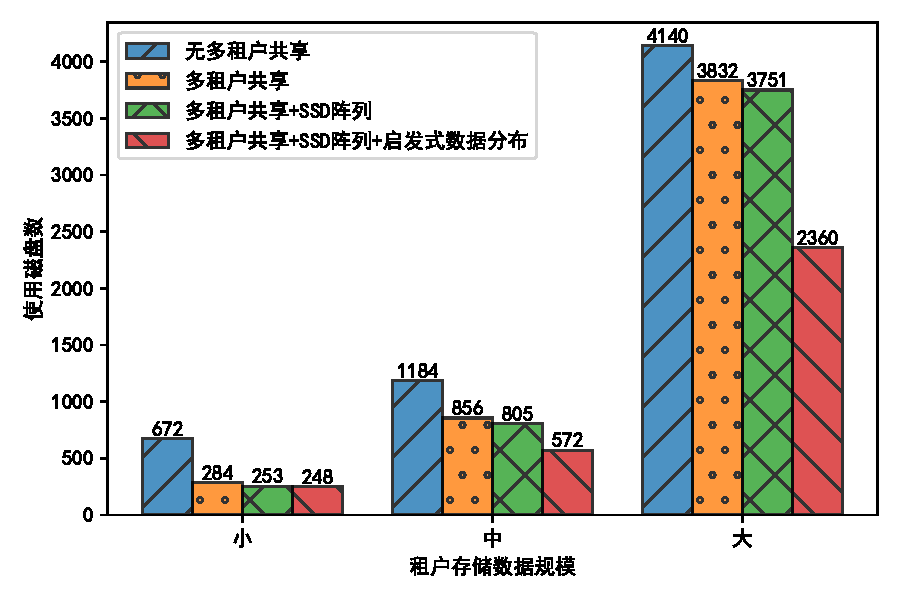
\includegraphics[width=0.8\textwidth]{thesis-sharing-savings.pdf}
  \caption{
        利用本系统提出的算法节约的SSD资源。
      }
  \label{fig:eval-sharing-savings}
\end{figure}
% !TeX root = ../main.tex

\chapter{总结}
% % !TeX root = ../main.tex

\chapter{浮动体}

\section{三线表}

三线表是《撰写手册》推荐使用的格式,如表~\ref{tab:exampletable}。
\begin{table}[h]
  \centering
  \caption{表号和表题在表的正上方}
  \label{tab:exampletable}
  \begin{tabular}{cl}
    \toprule
    类型   & 描述                                       \\
    \midrule
    挂线表 & 挂线表也称系统表、组织表,用于表现系统结构 \\
    无线表 & 无线表一般用于设备配置单、技术参数列表等   \\
    卡线表 & 卡线表有完全表,不完全表和三线表三种       \\
    \bottomrule
  \end{tabular}
  \note{注:表注分两种,第一种是对全表的注释,用不加阿拉伯数字排在表的下边,
    前面加“注:”;第二种是和表内的某处文字或数字相呼应的注,
    在表里面用带圈的阿拉伯数字在右上角标出,然后在表下面用同样的圈码注出来}
\end{table}

编制表格应简单明了,表达一致,明晰易懂,表文呼应、内容一致。
排版时表格字号略小,或变换字体,尽量不分页,尽量不跨节。
表格太大需要转页时,需要在续表上方注明“续表”,表头页应重复排出。



\section{插图}

有的同学可能听说“\LaTeX{} 只能使用 eps 格式的图片”,甚至把 jpg 格式转为 eps。
事实上,这种做法已经过时。
而且每次编译时都要要调用外部工具解析 eps,导致降低编译速度。
所以我们推荐矢量图直接使用 pdf 格式,位图使用 jpeg 或 png 格式。
\begin{figure}[h]
  \centering
  
\includegraphics[width=0.3\textwidth]{ustc-badge.pdf}
  \caption{图号、图题置于图的下方}
  \label{fig:badge}
  \note{注:图注的内容不宜放到图题中。}
\end{figure}

关于图片的并排,推荐使用较新的 \pkg{subcaption} 宏包,
不建议使用 \pkg{subfigure} 或 \pkg{subfig} 等宏包。



\section{算法环境}

模板中使用 \pkg{algorithm2e} 宏包实现算法环境。关于该宏包的具体用法,
请阅读宏包的官方文档。

\begin{algorithm}[h]
  \SetAlgoLined
  \KwData{this text}
  \KwResult{how to write algorithm with \LaTeX2e }

  initialization\;
  \While{not at end of this document}{
    read current\;
    \eIf{understand}{
      go to next section\;
      current section becomes this one\;
    }{
      go back to the beginning of current section\;
    }
  }
  \caption{算法示例1}
  \label{algo:algorithm1}
\end{algorithm}

注意,我们可以在论文中插入算法,但是插入大段的代码是愚蠢的。
然而这并不妨碍有的同学选择这么做,对于这些同学,建议用 \pkg{listings} 宏包。

% % !TeX root = ../main.tex

\chapter{数学}

\section{数学符号和公式}

《撰写手册》要求数学符号遵循 GB/T 3102.11—1993《物理科学和技术中使用的数学符号》
\footnote{原 GB 3102.11—1993,自 2017 年 3 月 23 日起,该标准转为推荐性标准。}。
该标准参照采纳 ISO 31-11:1992 \footnote{目前已更新为 ISO 80000-2:2019。},
但是与 \TeX{} 默认的美国数学学会(AMS)的符号习惯有所区别。
具体地来说主要有以下差异:
\begin{enumerate}
  \item 大写希腊字母默认为斜体,如
    \begin{equation*}
      \Gamma \Delta \Theta \Lambda \Xi \Pi \Sigma \Upsilon \Phi \Psi \Omega.
    \end{equation*}
    注意有限增量符号 $\increment$ 固定使用正体,模板提供了 \cs{increment} 命令。
  \item 小于等于号和大于等于号使用倾斜的字形 $\le$、$\ge$。
  \item 积分号使用正体,比如 $\int$、$\oint$。
  \item 行间公式积分号的上下限位于积分号的上下两端,比如
    \begin{equation*}
      \int_a^b f(x) \dif x.
    \end{equation*}
    行内公式为了版面的美观,统一居右侧,如 $\int_a^b f(x) \dif x$ 。
  \item
    偏微分符号 $\partial$ 使用正体。
  \item
    省略号 \cs{dots} 按照中文的习惯固定居中,比如
    \begin{equation*}
      1, 2, \dots, n \quad 1 + 2 + \dots + n.
    \end{equation*}
  \item
    实部 $\Re$ 和虚部 $\Im$ 的字体使用罗马体。
\end{enumerate}

以上数学符号样式的差异可以在模板中统一设置。
但是还有一些需要用户在写作时进行处理:
\begin{enumerate}
  \item 数学常数和特殊函数名用正体,如
    \begin{equation*}
      \uppi = 3.14\dots; \quad
      \symup{i}^2 = -1; \quad
      \symup{e} = \lim_{n \to \infty} \left( 1 + \frac{1}{n} \right)^n.
    \end{equation*}
  \item 微分号使用正体,比如 $\dif y / \dif x$。
  \item 向量、矩阵和张量用粗斜体(\cs{symbf}),如 $\symbf{x}$、$\symbf{\Sigma}$、$\symbfsf{T}$。
  \item 自然对数用 $\ln x$ 不用 $\log x$。
\end{enumerate}

模板中使用 \pkg{unicode-math} 宏包配置数学字体。
该宏包与传统的 \pkg{amsfonts}、\pkg{amssymb}、\pkg{bm}、
\pkg{mathrsfs}、\pkg{upgreek} 等宏包\emph{不}兼容。
本模板作了处理,用户可以直接使用 \cs{bm}, \cs{mathscr},
\cs{upGamma} 等命令。
关于数学符号更多的用法,参见 \pkg{unicode-math} 宏包的使用说明和符号列表
\pkg{unimath-symbols}。



\section{量和单位}

宏包 \pkg{siunitx} 提供了更好的数字和单位支持:
\begin{itemize}
  \item \num{12345.67890}
  \item \num{1+-2i}
  \item \num{.3e45}
  \item \num{1.654 x 2.34 x 3.430}
  \item \si{kg.m.s^{-1}}
  \item \si{\micro\meter} $\si{\micro\meter}$
  \item \si{\ohm} $\si{\ohm}$
  \item \numlist{10;20}
  \item \numlist{10;20;30}
  \item \SIlist{0.13;0.67;0.80}{\milli\metre}
  \item \numrange{10}{20}
  \item \SIrange{10}{20}{\degreeCelsius}
\end{itemize}



\section{定理和证明}

示例文件中使用 \pkg{amsthm} 宏包配置了定理、引理和证明等环境。
用户也可以使用 \pkg{ntheorem} 宏包。

\begin{definition}
  If the integral of function $f$ is measurable and non-negative, we define
  its (extended) \textbf{Lebesgue integral} by
  \begin{equation}
    \int f = \sup_g \int g,
  \end{equation}
  where the supremum is taken over all measurable functions $g$ such that
  $0 \le g \le f$, and where $g$ is bounded and supported on a set of
  finite measure.
\end{definition}

\begin{assumption}
The communication graph is strongly connected.
\end{assumption}

\begin{example}
  Simple examples of functions on $\mathbb{R}^d$ that are integrable
  (or non-integrable) are given by
  \begin{equation}
    f_a(x) =
    \begin{cases}
      |x|^{-a} & \text{if } |x| \le 1, \\
      0        & \text{if } x > 1.
    \end{cases}
  \end{equation}
  \begin{equation}
    F_a(x) = \frac{1}{1 + |x|^a}, \qquad \text{all } x \in \mathbb{R}^d.
  \end{equation}
  Then $f_a$ is integrable exactly when $a < d$, while $F_a$ is integrable
  exactly when $a > d$.
\end{example}

\begin{lemma}[Fatou]
  Suppose $\{f_n\}$ is a sequence of measurable functions with $f_n \geq 0$.
  If $\lim_{n \to \infty} f_n(x) = f(x)$ for a.e. $x$, then
  \begin{equation}
    \int f \le \liminf_{n \to \infty} \int f_n.
  \end{equation}
\end{lemma}

\begin{remark}
  We do not exclude the cases $\int f = \infty$,
  or $\liminf_{n \to \infty} f_n = \infty$.
\end{remark}

\begin{corollary}
  Suppose $f$ is a non-negative measurable function, and $\{f_n\}$ a sequence
  of non-negative measurable functions with
  $f_n(x) \le f(x)$ and $f_n(x) \to f(x)$ for almost every $x$. Then
  \begin{equation}
    \lim_{n \to \infty} \int f_n = \int f.
  \end{equation}
\end{corollary}

\begin{proposition}
  Suppose $f$ is integrable on $\mathbb{R}^d$. Then for every $\epsilon > 0$:
  \begin{enumerate}
    \renewcommand{\theenumi}{\roman{enumi}}
    \item There exists a set of finite measure $B$ (a ball, for example) such
      that
      \begin{equation}
        \int_{B^c} |f| < \epsilon.
      \end{equation}
    \item There is a $\delta > 0$ such that
      \begin{equation}
        \int_E |f| < \epsilon \qquad \text{whenever } m(E) < \delta.
      \end{equation}
  \end{enumerate}
\end{proposition}

\begin{theorem}
  Suppose $\{f_n\}$ is a sequence of measurable functions such that
  $f_n(x) \to f(x)$ a.e. $x$, as $n$ tends to infinity.
  If $|f_n(x)| \le g(x)$, where $g$ is integrable, then
  \begin{equation}
    \int |f_n - f| \to 0 \qquad \text{as } n \to \infty,
  \end{equation}
  and consequently
  \begin{equation}
    \int f_n \to \int f \qquad \text{as } n \to \infty.
  \end{equation}
\end{theorem}

\begin{proof}
  Trivial.
\end{proof}

\newtheorem*{axiomofchoice}{Axiom of choice}
\begin{axiomofchoice}
  Suppose $E$ is a set and ${E_\alpha}$ is a collection of
  non-empty subsets of $E$. Then there is a function $\alpha
  \mapsto x_\alpha$ (a ``choice function'') such that
  \begin{equation}
    x_\alpha \in E_\alpha,\qquad \text{for all }\alpha.
  \end{equation}
\end{axiomofchoice}

\newtheorem{observation}{Observation}
\begin{observation}
  Suppose a partially ordered set $P$ has the property
  that every chain has an upper bound in $P$. Then the
  set $P$ contains at least one maximal element.
\end{observation}
\begin{proof}[A concise proof]
  Obvious.
\end{proof}

% % !TeX root = ../main.tex

\chapter{引用文献的标注}

模板使用 \pkg{natbib} 宏包来设置参考文献引用的格式,
更多引用方法可以参考该宏包的使用说明。



\section{顺序编码制}

\subsection{角标数字标注法}

\ustcsetup{
  cite-style = super,
}
\noindent
\begin{tabular}{l@{\quad$\Rightarrow$\quad}l}
  \verb|\cite{knuth86a}|         & \cite{knuth86a}         \\
  \verb|\citet{knuth86a}|        & \citet{knuth86a}        \\
  \verb|\cite[42]{knuth86a}|     & \cite[42]{knuth86a}     \\
  \verb|\cite{knuth86a,tlc2}|    & \cite{knuth86a,tlc2}    \\
  \verb|\cite{knuth86a,knuth84}| & \cite{knuth86a,knuth84} \\
\end{tabular}


\subsection{数字标注法}

\ustcsetup{
  cite-style = inline,
}
\noindent
\begin{tabular}{l@{\quad$\Rightarrow$\quad}l}
  \verb|\cite{knuth86a}|         & \cite{knuth86a}         \\
  \verb|\citet{knuth86a}|        & \citet{knuth86a}        \\
  \verb|\cite[42]{knuth86a}|     & \cite[42]{knuth86a}     \\
  \verb|\cite{knuth86a,tlc2}|    & \cite{knuth86a,tlc2}    \\
  \verb|\cite{knuth86a,knuth84}| & \cite{knuth86a,knuth84} \\
\end{tabular}



\section{著者-出版年制标注法}

\ustcsetup{
  cite-style = authoryear,
}
\noindent
\begin{tabular}{l@{\quad$\Rightarrow$\quad}l}
  \verb|\cite{knuth86a}|         & \cite{knuth86a}         \\
  \verb|\citep{knuth86a}|        & \citep{knuth86a}        \\
  \verb|\citet[42]{knuth86a}|    & \citet[42]{knuth86a}    \\
  \verb|\citep[42]{knuth86a}|    & \citep[42]{knuth86a}    \\
  \verb|\cite{knuth86a,tlc2}|    & \cite{knuth86a,tlc2}    \\
  \verb|\cite{knuth86a,knuth84}| & \cite{knuth86a,knuth84} \\
\end{tabular}

\ustcsetup{
  cite-style = super,
}

% 注意,参考文献列表中的每条文献在正文中都要被引用。这里只是为了示例。
\nocite{*}


\backmatter
\bibliography{bib/ustc}  % 参考文献使用 BibTeX 编译
% \printbibliography       % 参考文献使用 BibLaTeX 编译

\appendix

% % !TeX root = ../main.tex

\begin{publications}

\section*{已发表论文}

\begin{enumerate}
\item A A A A A A A A A
\item A A A A A A A A A
\item A A A A A A A A A
\end{enumerate}

\section*{待发表论文}

\begin{enumerate}
\item A A A A A A A A A
\item A A A A A A A A A
\item A A A A A A A A A
\end{enumerate}

\section*{研究报告}
\begin{enumerate}
\item A A A A A A A A A
\item A A A A A A A A A
\item A A A A A A A A A
\end{enumerate}

\end{publications}


\end{document}
